%!TEX root = ../../Master.tex
\section{Existing systems} % (fold)
\label{sec:existing_systems}
In this chapter, the different commonly used navigation systems will be discussed and analysed in relative to their strengths and weaknesses.

\paragraph{Signs}
There are signs placed that mark different areas of the hospital. "Main entrance" and "Ambulance entrance"\cite{signs_hospital} signs can be used to mark key places that the visitor can navigate from\cite{art_Osborne}.
Interior signs are also places in the hospital. These painted to the walls, affixed to doors or windows\cite{signs_wall} and others hanging from the ceiling. These describe what room or hall the visitor is in. Some of these signs also contain information about where the different areas of the hospital can be located, often marked by a line of text followed up by a arrow pointing in a specified direction\cite{signs_hospital2}. If the hospital is made up by multiple buildings, they can be numbered in order to navigate people to specific buildings. 
A positive about the signs is that they can give a fast impression about where the different locations are.

The signs can be hard to spot if the  visitor is not familiar with the hospital, also a sign can be obstructed by other signs or if the room/hallway is filled with people. Another problem regarding the signs, is that they might be hard to use if the visitor have reading problems. If the one reading the sign cannot understand the language or is an illiterate, it becomes hard to find the information that is relevant\cite{signs_reading}. Too much information can also be displayed on signs so that it becomes confusing or hard to see the system behind the sign placements.
Also, if the visitor is in building A, and wants to visit a patient in building B floor 6. It could become a challenge to set up enough signs to guide the visitor to the right building and floor, without drowning the other visitors with non relevant information.

  \begin{figure}[ht!]
  \centering
  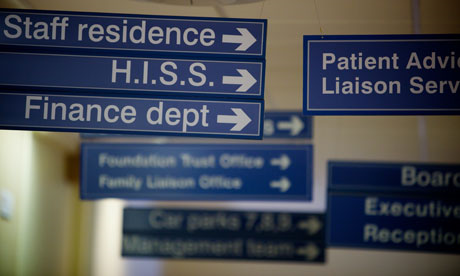
\includegraphics[width=90mm]{Alder-Hey-hospital-signs-007.png}
  \caption{A lot of signs showing different departments at a hospital\cite{signs_hospital}}
  \label{overflow}
  \end{figure}
  \begin{figure}[ht!]
  \centering
  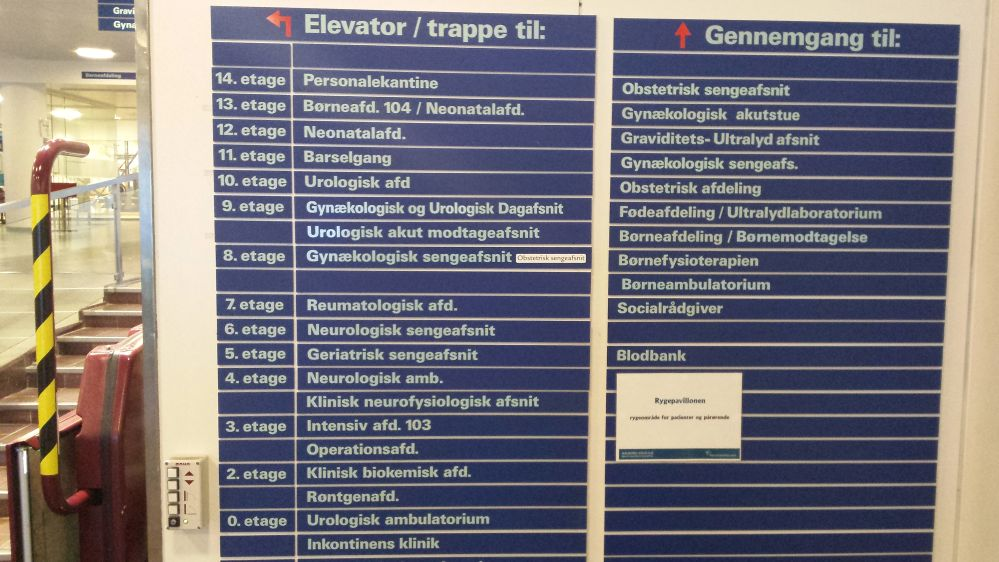
\includegraphics[width=90mm]{tavle.png}
  \caption{A signs that shows what is on the different floors at Sygeus nord}}
  \label{overflow}
  \end{figure}  
\paragraph{Human contact}

\paragraph{Maps}
Analog maps\cite{map} offers a top-down view of the hospital with all the different locations marked by text or colour\cite{art_Osborne}. The map can be painted on a wall\cite{wall_map} or found in a compact version meant to be carried around. The stationary maps sometimes have a red dot that marks where the reader is. By knowing the current position, the visitor should be able to navigate with more ease\cite{map_survey} as they will not have to look for something recognizable. If the building has multiple floors, the map will be split up into sections in order to cover all the rooms.
Maps are able to efficiency show hot spots and quickly gain a overview on the location\cite{pros_analog_map}.

A big problem with maps is they can become very complicated to get a overview of if they cover multiple floors \cite{map_confusing}. If the visitor is already inside the building, it can sometimes be difficult to figure out where they are corresponding to the map. If they are standing in a hallway it can be difficult to distinguish it from the others. 

  \begin{figure}[ht!]
  \centering
  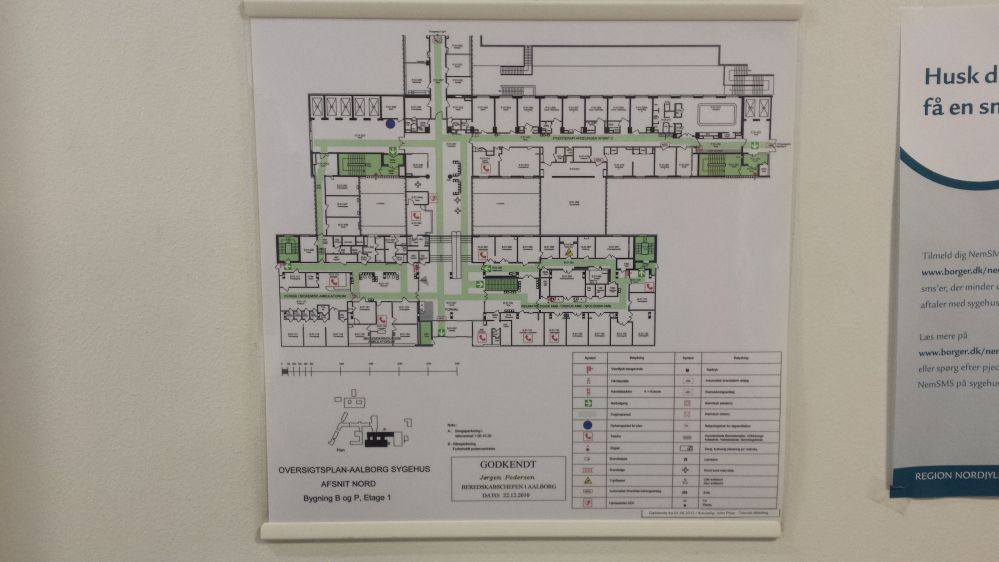
\includegraphics[width=90mm]{kortvaeg.png}
  \caption{A map on the wall at Sygehus nord}
  \label{overflow}
  \end{figure}
\paragraph{Colour coding}
Coloured stripes across the wall or floor that leads to the different areas of the hospital. In the entrance hall the visitors will see a wall with some lines of text with a coloured stripe behind it. One line might say "recovery" and if followed, will lead to the recovery department. Some departments also have an entire theme in a certain colour. In this way, it might become easier for some people to navigate the next time they visit, if they can remember the colours representing the department. 
Places that use this method of navigation would seamlessly offer an easy way of letting the visitors navigate.

If some rooms switches their function the stripes on the wall have to be repainted which will be a lot of work. If there are stripes leading to all the different departments, the information could potentially clutch up and become confusing. This method also shares a downside together with the signs, as people with reading disorder could have trouble with this form of navigation.
  \begin{figure}[ht!]
  \centering
  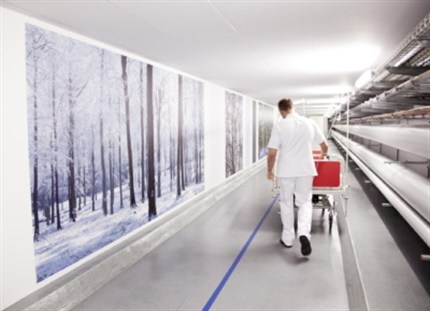
\includegraphics[width=90mm]{gang-vinter_430x311.png}
  \caption{A hall with a single colour at the floor}
  \label{overflow}
  \end{figure}
    \begin{figure}[ht!]
    \centering
    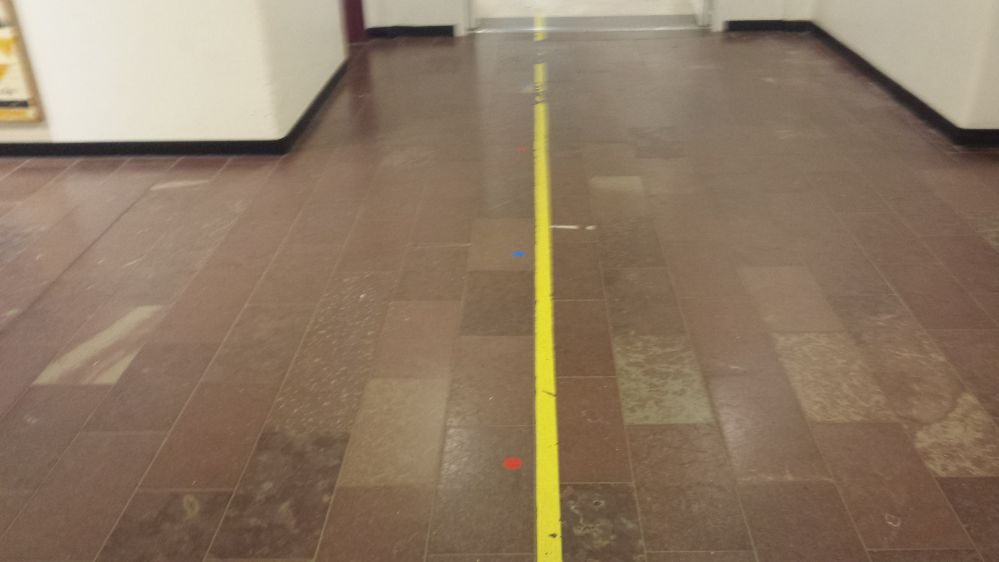
\includegraphics[width=90mm]{stribe2.png}
    \caption{Another example of colour coding, seen at Sygehus nord}
    \label{overflow}
    \end{figure}
\paragraph{Human contact}
\subsection{Phone}
Visitors are able to call the hospital's main number, and ask questions to a live operator. This can be done from any phone but there is no guarantee that a live operator is available.

The limitations regarding the phone, are high as the informer is limited by only having his/her voice as their tool. Miscommunication can occur as directions only can be delivered by words. As said before, this form of navigation strictly depends on an assigned personal to answer the phone. If no one is at the phone, it becomes utterly useless.
If the service is used often, more than one employee might be assigned to the phone. It could become an expensive service if there is a dedicated staff assigned to the phone. 

\subsection{Porter}
The porter helps patients\cite{porter} and visitors get around at the hospital. The porter helps visitors find available beds if they have to stay at the hospital overnight \cite{ugd_port}. An employee would probably be able to navigate at their working place with ease.

The porter has other tasks he/she needs to attend to and will not always be available. Also, if the visitor have used the porter to get to a certain room, and wants to leave an hour later, they might not know where to find a new one. 

\subsection{Receptionist}
The receptionist can answer questions from the visitors\cite{job}. Very much like the phone, but with some key differences. The phone is more accessible as the one calling does not need to be at the hospital. The receptions has an advantage of being more precise. There will be less confusion as body language can be used in the answering of the question\cite{body_vs_phone}.

If the visitor arrives at an entrance different from the main one, they might not know where the receptionist is if they need help. The information received from the receptions have to be memorized when the visitor ventures away from the desk. This means that directions could become hard to remember if they have to get to distant location inside the building. A way the receptionist could help the visitor remember, would be to write a note but even so the text could be misunderstood or in other ways mixed up.

  \begin{figure}[ht!]
  \centering
  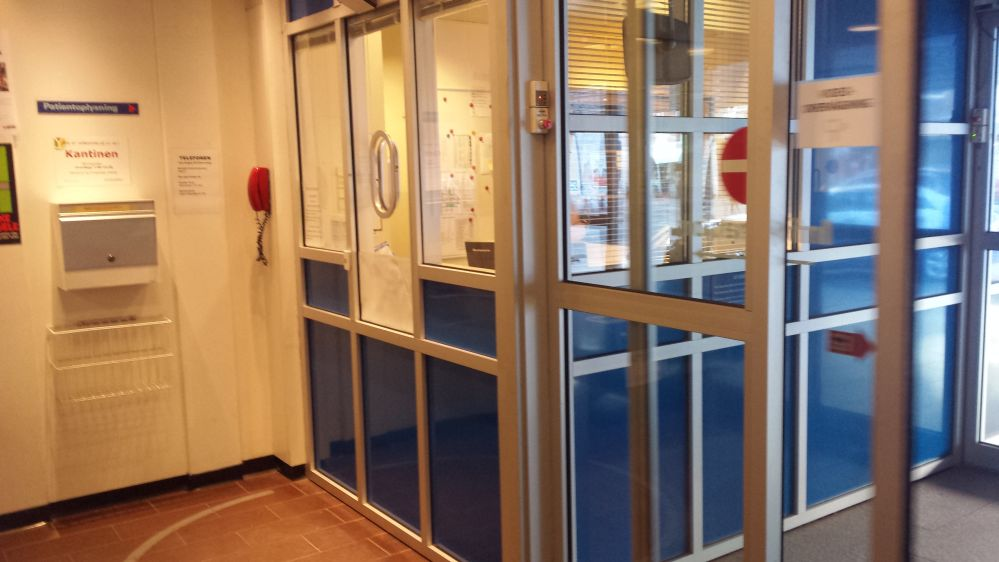
\includegraphics[width=90mm]{reception.png}
  \caption{A receptionist booth, seen at Sygehus nord}
  \label{overflow}
% section existing_systems (end)